\documentclass{report}


%German setting
\usepackage{ngerman}
\usepackage[latin1]{inputenc}
\usepackage[official]{eurosym}
\usepackage[T1]{fontenc}

\usepackage{graphicx}  % Include grafics
\usepackage{grffile}   % support special grafic names
\usepackage{listings}  % Source code
\lstset{
    breaklines=true,
}

%\usepackage{titleref}  %- don't work error: Command titeref alread defined!
\usepackage{html}

\pagestyle{plain}





\setcounter{tocdepth}{3}
\setcounter{secnumdepth}{3} 

\providecommand{\versionnumber}{1.1}

\title{Beispiel E-Book}
\author{Martin Strohmayer\\m.stroh@ymail.com\\ \url{http://evil.hn.vc}}
\date{Version \versionnumber \\\today \\E-Book Edition}

\begin{document}

\maketitle

\tableofcontents

\chapter*{Vorwort}
Dieses Buch dient zur Veranschaulichung und als Vorlage f�r E-Books die mit Latex erzeugt werden.
Dieses Buch steht unter der CC0 1.0 Lizenz und kann bedingungslos als Vorlage f�r E-Books von jedermann verwendet werden. Dies gilt auch f�r alle enthaltenen Bilder, Skripte und Texte.\\ 
CC0 Lizenz siehe \url{https://creativecommons.org/publicdomain/zero/1.0/}.\\
Die Quell-Dateien des E-Books stehen auf GitHub zur Verf�gung \url{https://github.com/mstroh76/Beispiel-EBook}.

\clearpage

\chapter{Formatierungen}

\section{Schrifttyp}

\paragraph{"`console"'}

\begin{console}
lspci | grep VGA
\end{console}


\paragraph{"`screen"'}

\begin{screen}
00:01.1 VGA compatible controller: Advanced Micro Devices [AMD] Geode LX Video
\end{screen}

\paragraph{"`consolesmall"'}

\begin{consolesmall}
uname -a
\end{consolesmall}

\paragraph{"`screensmall"'}

\begin{screensmall}
Linux A220 3.16.0-0.bpo.4-586 #1 Debian 3.16.7 (2015-08-08) i586 GNU/Linux
\end{screensmall}

\paragraph{"`filename"' und "`file"'}~\\

\filename{/etc/debian\_version}
\begin{file}
7.9
\end{file}

\section{Adressen und Pfade}

\paragraph{"`url"'}~\\

\url{http://www.amazon.de/kindle/dp/B00JGEEZOS}\\

\paragraph{"`urlsmall"'}~\\

\urlsmall{http://play.google.com/store/books/details/Martin_Strohmayer_Raspberry_Pi_Projekte?id=d6KAAwAAQBAJ}

\paragraph{"`path"'}~\\

\path{C:\Program Files (x86)\Steam\SteamApps\common\}\\

\paragraph{"`folder"'}~\\

\folder{C:\Program Files (x86)\Steam\SteamApps\common\}\\


\chapter{Quellcode}

\paragraph{"`lstinputlisting"'}~\\

\lstset{language=C, caption='HelloWord.c' C-Quellcode-Datei, label=lst:HelloWord_c, showstringspaces=false, showtabs=false, tabsize=2 }
\lstinputlisting{files/HelloWord.c}

\paragraph{"`lstlisting"'}~\\

\lstset{language=Bash, caption='HelloWord.sh' Shell-Skript, label=lst:HelloWord_sh, showstringspaces=false, showtabs=false, tabsize=2 }
\begin{lstlisting}
#!/bin/bash
echo "Hello, World!"
\end{lstlisting}

\chapter{Aufz�hlungen}

\section{Beschreibung} \label{sec:Beschreibung}

\begin{description}
\item[console] Definiert Eingaben, die �ber die Konsole bzw. Kommandozeile eingeben werden m�ssen.  
\item[screen] Definiert Ausgaben am Bildschirm (zumeist auch auf der Konsole).
\item[filename] Definiert einen Dateinamen, der zumeist vor einem file-Bereich verwendet wird.
\item[file] Definiert Texte, die sich in einer Datei befinden.
\item[url] Definiert Internetadressen.
\end{description}


\section{Nummeriert} \label{sec:Nummeriert}

\begin{enumerate}
\item Erstens
\item Zweitens
\item Drittens
\end{enumerate}

\section{Einzelpunkte} \label{sec:Einzelpunkte}

\begin{itemize}
\item Erstens
\item Zweitens
\item Drittens
\end{itemize}


\section{Gemischt} \label{sec:Gemischt}

\begin{description}
   \item[Variante 1] Aufz�hlung nummeriert
   \begin{enumerate}
      \item Unterebene Aufz�hlung nummeriert 1
      \begin{enumerate}
         \item Erstens
         \item Zweitens
				 \item Drittens
      \end{enumerate}
      \item Unterebene Aufz�hlung nummeriert 2
      \begin{enumerate}
         \item Erstens
         \item Zweitens
				 \item Drittens
      \end{enumerate}
   \end{enumerate}
	
   \item[Variante 2] Aufz�hlung Einzelpunkte
   \begin{itemize}
      \item Unterebene Aufz�hlung Einzelpunkte 1
      \begin{itemize}
         \item Erstens
         \item Zweitens
				 \item Drittens
      \end{itemize}
      \item Unterebene Aufz�hlung Einzelpunkte 2
      \begin{itemize}
         \item Erstens
         \item Zweitens
				 \item Drittens
      \end{itemize}			
   \end{itemize}
\end{description}

\chapter{Tabelle} \label{chap:Tabelle}

\section{Schmall}

\begin{table}[h]
\label{tab:schmall}
\centering
\begin{tabular}{|l|c|c|c |}
\hline
                        & \textbf{Taktfrequenz} & \textbf{CPU-Kerne} &  \textbf{RAM} \\
                        & MHz &  &  MB \\
\hline
\textbf{Raspberry Pi}   & 700   & 1 & 512\\
\hline
\textbf{Raspberry Pi 2} & 900   & 4 & 1024\\
\hline
\textbf{Banana Pi}      & 1000  & 2 & 1024\\
\hline
\textbf{Orange Pi PC}      & 1600  & 4 & 1024\\
\hline
\end{tabular}
\end{table}

\section{Breit}

\begin{table}[h]
\label{tab:breit}
\centering
\begin{tabular}{|l|c|c|c|c|c|}
\hline
\textbf{} & \textbf{Einheit}  & \textbf{Raspberry Pi} & \textbf{Raspberry Pi 2} & \textbf{Banana Pi}  & \textbf{Orange Pi}\\
\hline
Taktfrequenz & MHz & 700 & 900 & 1000 & 1600\\
\hline
CPU-Cores &	& 1 & 4 & 2 & 4\\	
\hline
RAM & MB & 512 & 1024 & 1024 & 1024\\	
\hline
\end{tabular}
\end{table}

\chapter{Grafik}

\section{PNG-Grafikdatei}

\begin{figure}[ht]
  \centering
  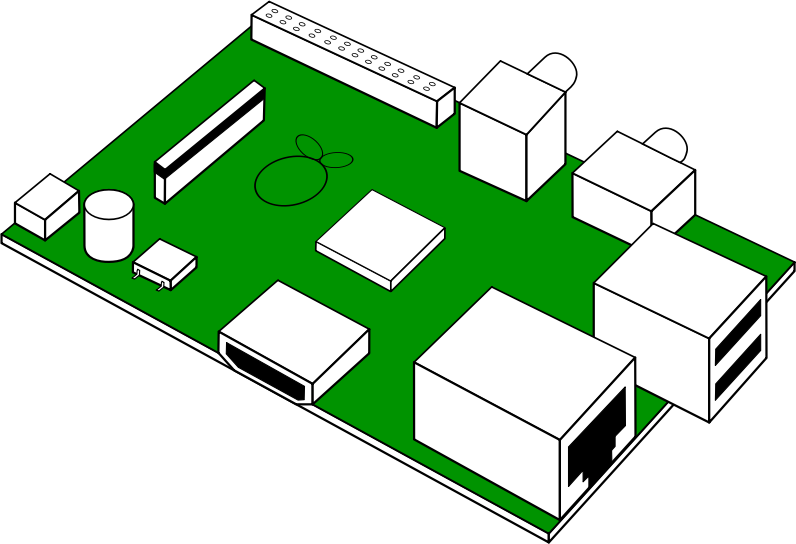
\includegraphics[scale=0.13]{images/raspberry-pi-pcb-800px.png}
  \caption{Raspberry Pi Clipart}
  \label{fig:Raspberry_Pi_Clipart}
\end{figure}


\section{JPG-Grafikdatei}

\begin{figure}[ht]
  \centering
  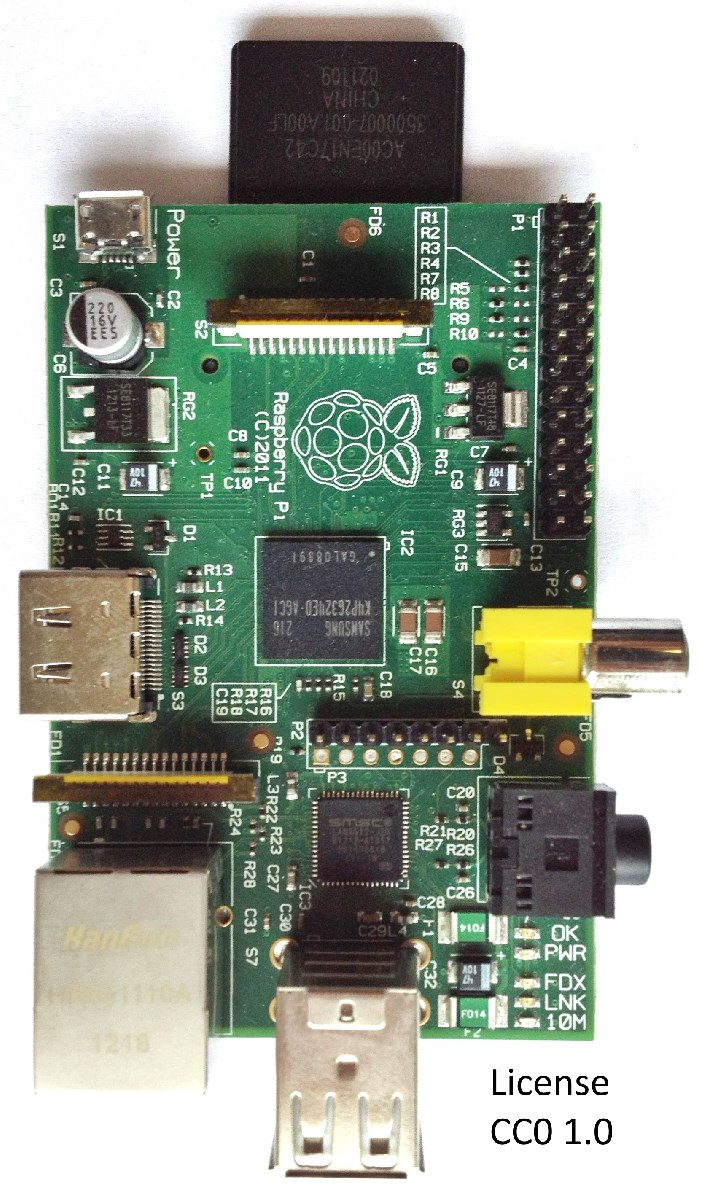
\includegraphics[scale=0.12]{images/Raspberry_Pi.jpg}
  \caption{Raspberry Pi Foto}
  \label{fig:Raspberry_Pi_Foto}
\end{figure}


\chapter{Mathematik (Formeln)}

\section{Formeln direkt darstellbar}

\begin{Large}
$ U_{2} = U / ( R_{1} + R_{2} ) \cdot R_{2} $ \\

$ P = I_{f}^{2} \cdot R $ \\

$ s_{xy} = \int_{x}^{y} (a \cdot t + V_{0}) \cdot dt $

\end{Large}

\section{Formeln als Grafik}

\paragraph{Bruch}~\\

\begin{Large}
$ I_{f} = \frac{U_{f}}{R} \label{eq:Bruch} $ \\
\end{Large}


\paragraph{Wurzel}~\\

\begin{Large}
$ c=\sqrt[]{a^{2}+b^{2}} \label{eq:Wurzel} $ \\
\end{Large}


\paragraph{Explizit als Grafik formatiert}~\\

\begin{Large}
$$ U_{2} = U / ( R_{1} + R_{2} ) \cdot R_{2} $$\\
\end{Large}


\section{Griechische Buchstaben}

$\Gamma \dots$ Gamma\\
$\Delta \dots$ Delta\\
$\Theta \dots$ Theta\\
$\Lambda \dots$ Lambda\\
$\Xi \dots$ Xi\\
$\Pi \dots$ Pi\\
$\Sigma \dots$ Sigma\\
$\Upsilon \dots$ Sigma\\
$\Phi \dots$ Ypsilon\\
$\Psi \dots$ Psi\\
$\Omega \dots$ Omega\\
$\alpha \dots$ Alpha\\
$\beta \dots$ Beta\\
$\gamma \dots$ Gamma\\
$\delta \dots$ Delta\\
$\epsilon \dots$ Epsilon\\
$\varepsilon \dots$ Epsilon (varepsilon)\\
$\zeta \dots$ Zeta\\
$\eta \dots$ Eta\\
$\theta \dots$ Theta\\ 	
$\vartheta \dots$ Theta (vartheta)\\
$\iota \dots$ Iota\\
$\kappa \dots$ Kappa\\
$\lambda \dots$ Lambda\\ 	
$\mu \dots$ My\\
$\nu \dots$ Ny\\
$\xi \dots$ Xi\\
$\pi \dots$ Pi\\
$\varpi \dots$ Pi (varpi)\\
$\rho \dots$ Rho\\
$\varrho \dots$ Rho (varrho)\\
$\sigma \dots$ Sigma\\
$\varsigma \dots$ Sigma (varsigma)\\
$\tau \dots$ Tau\\
$\upsilon \dots$ Ypsilon\\ 	
$\phi \dots$ Phi\\
$\varphi \dots$ Phi (varphi)\\
$\chi \dots$ Chi\\
$\psi \dots$ Psi\\
$\omega \dots$ Omega\\


\section{Operatoren}

%https://de.wikipedia.org/wiki/Liste_mathematischer_Symbole

$\le \dots$ Gr��er als oder gleich\\
$\ge \dots$ Kleiner als oder gleich\\
$\approx \dots$ Ungef�hr\\
$\neq \dots$ Ungleich\\
$\ll \dots$ Wesentlich Gr��er\\
$\gg \dots$ Wesentlich Kleiner\\
$\pm \dots$ Plusminus\\
$\mp \dots$ Minusplus\\
$\times \dots$ Multiplikator\\ 
$\cdot \dots$ Multiplikator\\


\chapter{Verlinkungen}

\section{Kapitel}

Im Kapiel \ref{chap:Tabelle} \titleref{chap:Tabelle} kann die Darstellung von Tabellen �berpr�ft werden.  

\section{Unterkapitel}

Im Unterkapitel \ref{sec:Nummeriert} \titleref{sec:Nummeriert} wird die Formatierung einer nummerierten Aufz�hlung dargestellt.

\section{Grafik}

Raspberry Pi als JPG-Grafik siehe Abbildung \ref{fig:Raspberry_Pi_Foto} \titleref{fig:Raspberry_Pi_Foto}.\\
Raspberry Pi als PNG-Grafik siehe Abbildung \ref{fig:Raspberry_Pi_Clipart} \titleref{fig:Raspberry_Pi_Clipart}.\\


\section{Quellcode}

Kompiliert man die Datei \ref{lst:HelloWord_c} \titleref{lst:HelloWord_c} mit gcc erh�lt man eine ausf�hrbare Datei.\\
Das Skript von \ref{lst:HelloWord_sh} \titleref{lst:HelloWord_sh} kann direkt ausgef�hrt werden.


\section{Tabelle}

Die Tabelle \ref{tab:schmall} \titleref{tab:schmall} kann komplett am Bildschirm des Kindle Paperwhite dargestellt werden.

\section{Formel}

Die Formel \ref{eq:Bruch} \titleref{eq:Bruch} kann nur als Grafik dargestellt werden.

\chapter*{Anhang}

\section*{Versionshistorie}
\lhead{}
\chead{}
\rhead{ANHANG}

\begin{itemize}
\item 1.1
	\begin{itemize}
	\item Versionshistorie hinzugef�gt
	\end{itemize}
\end{itemize}

\section*{Danksagung}
\lhead{}
\chead{}
\rhead{ANHANG}

Ich bedanke mich bei allen Mitwirkenden.

\section*{Impressum}
\lhead{}
\chead{}
\rhead{ANHANG}

% Anpassen!
Autor, Eigenverlag: Martin Strohmayer (m.stroh@ymail.com)\\
Herstellungsort: Anthauerweg 15A, 8054 Graz, �sterreich\\





\end{document}
%EOF
